\chapter{Relación en TC}
Utilizaremos un dispositivo llamado par ordenado (p.o).\\
\textbf{Notación: }$(a,b)$\\
$(a,b)\not=\lbrace a,b\rbrace$

El orden es relevante $(a,b)\not=(b,a)$\\
$(a,b) \mbox{ es igual a (c,d) si } a=c\land b=d$\\
\textbf{Producto cartesiano}
$A\times B=\{ (a,b)/a\in A \land b\in B\}$

\section{Relación Binaria}
\textbf{Ejemplo: }
\begin{enumerate}
\item Si $A=\lbrace1,3,9\rbrace \quad B=\lbrace b,c,d\rbrace \\
	R_1=\lbrace (1,b),(1,c),(3,d),(9,d)\rbrace \subset A\times B$
\item $R_2=\lbrace (i,j)/ i,j\in \mathds{N} \land i<j\rbrace \subset \mathds{N}\times\mathds{N}$
\end{enumerate}

En una relación binaria $R\subseteq A\times B$ definimos:
$dom(R)=\lbrace a/\exists b\in B ,\quad (a,b)\in R\rbrace\\
ran(R)=\lbrace b/\exists a\in A ,\quad (a,b)\in R\rbrace\\
\mbox{Hay dos relaciones unarias basicas}\\
R^{-1}=\lbrace(b,a)/(a,b)\in R\rbrace\\
R^C= A\times B= R$\\
Una operación importante es la composición $R_2\, \circ R_1$ definida para el caso en que $ran(R_1)\subset dom(R_2)$\\
$R_2oR_1=\lbrace (x,z)/\exists y\; (x,y)\in R_1 \land (y,z)\in R_2\rbrace$\\
Si $R\subseteq S\times S$ para un subconjunto S entonces diremos que ''R es una relación en S''. La relación identidad.\\
$I_s=\lbrace (a,a)/a\in S\rbrace$\\
Sea S una relación en S definimos.\\

Las potencias $R^i$ por:\\
$R^o=I_s \quad R^{i+1}=RoR^i \quad i\geq 0$\\

La clausura transitiva.\\
$R^+=\bigcup_{i=1}^\infty R^i$\\

La clausura transitiva y reflexiva. \\

$R^*= \bigcup_{i=0}^\infty R^i$

\section{Propiedades Básicas de las relaciones binarias}
Una relación binaria $R\subseteq S\times S$ se llama:\\
Reflexiva: Si $a\in S \rightarrow (a,a)\in R$\\
Simétrica: Si $(a,b)\in R\rightarrow(b,a)\in R$\\
Antisimétrica: Si $(a,b)\in R\land a\not=b \rightarrow(b,a)\not\in R$\\
Transitiva: Si $(a,b)\in R \land (b,c)\in R \rightarrow(a,c)\in R$

\textbf{Definición: } \\
Una relación R se dirá:
\begin{itemize}
\item De equivalencia, si es reflexiva,simétrica y transitiva.
\item Un orden parcial si es reflexiva, antisimétrica y transitiva.
\item Un orden total si R es un orden parcial $\forall a,b \in S \, \lor \, (a,b)\in R \lor (b,a)\in R$
\end{itemize}

\textbf{Definición: }Si R es una relación de equivalencia en S y $a\in S$ entonces el conjunto.\\
$[a]=\lbrace b/(a,b)\in R\rbrace$\\
Se le llama la clase de equivalencia de a respecto a la relación R.

\textbf{Lema: }Si R es una relación de equivalencia en S y $a,b\in S$ las proposiciones son equivalentes:
\begin{enumerate}
\item $(a,b)\in R$
\item $[a]_R=[b]_R$
\item $[a]_R \cap [b]_R \not= \phi$
\end{enumerate}

\section{Representación de las Relaciones}
Dos de las mas importantes representaciones para relaciones son las matrices booleanas y los grafos dirigidos.\\
Sea $R\subseteq S\times S$ una relación binaria, donde $|S|=n$. Esta puede representarse mediante una matriz booleana $n \times n$. $M_R$ que estará formada por ''1'' si $(a,b)\in R$ y ''0'' si $(a,b)\not=R$.\\

\textbf{Ejemplo: } Sea R la relación.\\
$R=\lbrace(0,0),(0,1),(1,2),(1,3),(2,4),(2,5),(3,6),(3,7),\\
 \quad\quad(4,0),(4,1),(5,2),(5,3),(6,4),(6,5),(7,6),(7,7)\rbrace$\\
Su matriz booleana es:\\
$$\begin{pmatrix}
1 & 1 & 0 & 0 & 0 & 0 & 0 & 0\\
0 & 0 & 1 & 1 & 0 & 0 & 0 & 0\\
0 & 0 & 0 & 0 & 1 & 1 & 0 & 0\\
0 & 0 & 0 & 0 & 0 & 0 & 1 & 1\\
1 & 1 & 0 & 0 & 0 & 0 & 0 & 0\\
0 & 0 & 1 & 1 & 0 & 0 & 0 & 0\\
0 & 0 & 0 & 0 & 1 & 1 & 0 & 0\\
0 & 0 & 0 & 0 & 0 & 0 & 1 & 1\\
\end{pmatrix}$$

También podemos usar un grafo dirigido $G_R=(V,E)$ donde $V=dom(R)\cup ran(R)$ y $E=\lbrace(a,b)/(a,b)\in R\rbrace$\\
\begin{figure}
\centering
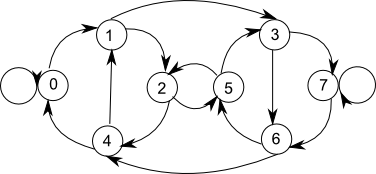
\includegraphics[width=0.5\textwidth]{img_2_1.png} 
\caption{Grafo dirigido}
\end{figure}


Si $M_{R_i} \quad i=1,2$ es una representación en matriz booleana de la relación $R_i$, entonces tenemos:

$$M_{R_1\cup R_2}=M_{R_1}\lor M_{R_2}\quad ; \quad
M_{R_1\cap R_2}=M_{R_1}\land M_{R_2}$$

\section{Posets}
Un conjunto S junto con una relación de orden parcial R se denomina un conjunto parcialmente ordenado o Poset y se le denota por $(S,R)$. En el caso de los Posets se usa la notación $aRb$ para indicar que $(a,b)\in R$.\\
\textbf{Ejemplo: } Si $\backslash$ denota la relación de divisibilidad entre enteros, entonces el par $(\mathds{N},\backslash)$ es un poset.\\
\textbf{Ejemplo: }\\
$\begin{array}{rl}7\in \mathds{N}, (7,7)\in \backslash \quad & reflexiva.\\
(6,2)\in \backslash \land 6\not=2 \; pero\; (2,6)\not\in \backslash \quad & antisimetrica.\\
(16,8)\in R \land (8,2)\in R \rightarrow (16,2)\in R \quad & transitiva.\end{array}$\\
 
Si A es cualquier conjunto, entonces $(2^A,\subseteq)$ es también un poset. Los posets pueden ser representados gráficamente mediante los diagramas Hasse. Estos están basados en el hecho que si $aRb \land bRc$ en un Poset (S,R) entonces $aRc$.\\
Sea (S,R) un poset. Denotamos $R_H \subseteq R$ la relación definida como sigue: $aR_H b$ si y solo si aRb y no hay $a\not=c\not=b$ tal que aRc y cRb.\\
En otras palabras $R_H$ es el conjunto mas pequeño con $R_H^*=R$.\\
\textbf{Ejemplo: }Sea $S=\lbrace 0,1,3\rbrace \; y \; R =\subseteq$, graficaremos el Poset $(2^S, \subseteq)$\\
$2^S=\lbrace \phi,\lbrace 0\rbrace,\lbrace 1\rbrace,\lbrace 2\rbrace,\lbrace 0,1\rbrace,\lbrace 0,2\rbrace,\lbrace 1,2\rbrace, S\rbrace$

\begin{figure}
\centering 
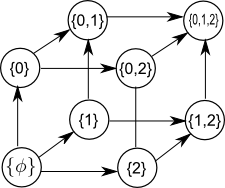
\includegraphics[width=0.35\textwidth]{img_2_2.png}
\caption{Gráfico del Poset}
\end{figure}

\section{Funciones}
El conjunto $f\subset A\times B$ es una función si:
\begin{itemize}
\item $Dom(f)=A$
\item Si $(x,y),(x,z)\in f \; entonces\; y=z$
\end{itemize}
Esto significa que para todo elemento x en A, existe un único y tal que $(x,y)\in f$.\\
\textbf{Notación: } $f:A\rightarrow B\\
					y=f(x)\quad(x,y)\in f$
					
A una función de éstas características la denominaremos función total.\\

\textbf{Teorema: }Sean las funciones $f:A\rightarrow B\; y\; g:A\rightarrow B$ Entonces $f=g$ si $f(x)=g(x) \forall x\in A$.

\subsection{Función Parcial}
Una relación $f\subseteq A\times B$ se denomina función parcial si:
\begin{itemize}
\item $Dom(f)\subseteq A$
\item Si $(x,y),(x,z)\in f\; entonces\; y=z$
\end{itemize}

\subsection{Imagen}
Sea $f:A\rightarrow B$ una función. Si $X\subseteq A$ se dice la imagen de X bajo f a : $f(x)=\lbrace y\in B/ y=f(x) ; para\; x\in X\rbrace$

\subsection{Imagen Inversa}
Sea $Y\subseteq B$, la imagen inversa de Y bajo f es: $f^{-1}(Y)=\lbrace x\in A / f(x)=y$ para algún $y\in Y\rbrace$

\textbf{Definición: } Sea $f:A\rightarrow B$ una función. Su rango es: $\lbrace f(x)/x\in A\rbrace$ que es un subconjunto del codominio B.

\subsection{Tipos Especiales de Funciones}
Sea $f:A\rightarrow B$ una función.
\begin{enumerate}
\item \textbf{Función Inyectiva: }f es inyectiva ó 1 a 1 si cumple:\\
	Para cualquier $(x,z)\in f \land (y,z)\in f\Rightarrow x=y$ o equivalente: si $f(x)=f(y) \Rightarrow x=y$
\item \textbf{Función Sobreyectiva: }f es sobreyectiva si su rango es todo el conjunto B o equivalente. $\forall y\in B, \exists x\in A / y=f(x)$
\item \textbf{Función Biyectiva: }Si f es a la vez inyectiva y sobreyectiva se dirá biyectiva. Cuando f es una biyección, $f^{-1}:B\rightarrow A$ es una función. La función inversa $f^{-1}:B\rightarrow A$ satisface:\\
$f^{-1}(f(x))=x \land f(f(f^{-1}(x))=y$
\end{enumerate}

\textbf{Ejemplo: }Para las siguientes funciones indique si son inyectivas y/o sobreyectivas.
\begin{enumerate}
\item $f:\mathds{N}\rightarrow \mathds{N} / f(n)=n$
\item $g:\mathds{N}\rightarrow \mathds{Z} / g(n)=n+1$
\item $h:\mathds{R}\rightarrow \mathds{R} / h(x)=x^2$
\end{enumerate}

\textbf{Solución: }Analizando cada uno de los casos.
\begin{itemize}
\item f es inyectiva, f es sobreyectiva.
\item g es inyectiva pero no sobreyectiva.
\item Si $h(x)=h(y)\\
			x^2=y^2\\
			\rightarrow x=y \lor x=-y$, entonces h no es inyectiva.
\item Si $y=-8, \not\exists x\in \mathds{R} / h(x)=y$ , entonces h no es sobreyectiva.
\end{itemize}

\section{Composición de Funciones}
Sean $f:A\rightarrow B \land g:C\rightarrow D$ definimos $g\circ f: A\rightarrow D$\\



$g\circ f(x)= \left \{  \begin{array}{rp{1cm}l} g(f(x)) & &x\in Dom\, f \land f(x)\in Dom\, g
				\\	indefinido & &\mbox{para otros casos}\end{array}\right.$\\

En general $f\circ g\not=g\circ f$\\

\textbf{Ejemplo: }Sean: $$\begin{array}{l} f:\mathds{Z}\rightarrow \mathds{N}/f(n)=|n|+1 \\
										g:\mathds{N}\rightarrow\mathds{Z}/g(n)=1-n\end{array}$$
Halle $f\circ g, g\circ f$.